\documentclass[problems]{esg8022pset} 
\usepackage{amsmath}
\usepackage{amssymb}
\usepackage{enumerate}
\usepackage{graphicx}
\usepackage{hyperref}
\usepackage{mathtools}
%\usepackage[per-mode=symbol]{siunitx} %If this line is giving you trouble, try replacing per-mode with per
%use inter-unit-separator={}\cdot{} ?
\providecommand{\uvec}[1]{{\hat{\bf{#1}}}}
%\usepackage{pgf,tikz}
%\usetikzlibrary{arrows}
\usepackage{wasysym}
\usepackage{subfig}
\makeatletter
\newcommand{\interitemtext}[1]{%
  \begin{list}{}
   {\itemindent=0mm\labelsep=0mm
   \labelwidth=0mm\leftmargin=0mm
   \addtolength{\leftmargin}{-\@totalleftmargin}}
    \item #1
  \end{list}
}
\makeatother
\renewcommand{\d}{\,d}
\providecommand{\norm}[1]{\lVert#1\rVert}
\DeclareMathOperator{\curl}{curl}

\AtBeginDocument{%
  % Apologies to any future editor on the inconsistencies in TeX code and the unnecessary braces.  I'm aggregating previously typeset problems, and didn't think it worth my time to improve the quality of TeX code in ways that won't make any difference to the typeset material. -Jason Gross (jgross@mit.edu)
}%
\classname{Physics 8.022} \semester{Spring 2011} 
\problemsetnumber{10}
\date{\today }
\duedate{Wednesday, May 4, 10 \textsc {am} IN CLASS}
\readingassignment{}
\problemsettitle{Maxwell's equations, waves}
\begin{document}
\section{Problem \thesection: Discovery of magnetic charge}
  You discover magnetic charge.  The units of magnetic charge density,
  $\mu$, are chosen such that $\vec\nabla\cdot\vec B = 4\pi\mu$.

  \begin{enumerate}[(a)]
    \item When this magnetic charge is in motion,
      there is a ``magnetic current density'' $\vec{L} = \mu \vec{v}$.  In
      analogy to electric charge density and electric current densities,
      write down the equation of continuity for magnetic charge.
    \item What do Maxwell's equations become with this
      new charge? \par\noindent
      Hint: The following vector identity may be useful: $\vec\nabla\cdot(\vec{\nabla}\times\vec{F}) = 0$ for any $\vec{F}$.
  \end{enumerate}
\section{Problem \thesection: Magnetic field of a moving charge}
  A charge $q$ moving
  along the $x$-axis at constant speed $v \ll c$.  When it is at $x =
  -d$, what is the magnetic field at $(x,y,z) = (0,r,0)$?

  \begin{enumerate}[(a)]
    \item Solve this first using Biot-Savart.  (Hint:
      the current from the moving charge isn't particularly well defined.
      However, B-S only needs the combination $I\,dl = (dq/dt)\,dl = dq\,
      (dl/dt) \simeq q_{\text{pt charge}}(dl/dt)$.  Sloppy physicist calculus
      in action!)
    \item Now solve this using displacement current.
      Look at a circle of radius $r$ centered at the origin and passing
      through the point $(0,r,0)$.  By symmetry, $\vec B$ will be constant
      on this circle and oriented in the tangential direction.  Find a
      surface which has this circle as a boundary and for which $\int \vec
      E\cdot d\vec a$ is simple.  Evaluate this flux, apply the
      ``generalized'' form of Ampere's law (integral formulation) and you're
      there.
  \end{enumerate}

  \noindent Note, there's a third way: Lorentz transform from the
  rest frame electric field.  All
  three answers should agree, at least in the limit $v \ll c$.
  \clearpage
\section{Problem \thesection: General questions}
  \begin{flalign*}
    \text{I. } \oiint_{\substack{\text{closed} \\ \text{surface}}} \vec{E} \cdot d\vec{a} & = 4\pi q_{\text{enclosed}} &
    \text{II. } \oiint_{\substack{\text{closed} \\ \text{surface}}} \vec{B} \cdot d\vec{a} & = 0 &
    \text{III. } \oint\limits_{\substack{\text{closed} \\ \text{loop}}} \vec{E} \cdot d\vec{s} & = -\frac{1}{c}\frac{d}{dt}\iint_{\substack{\text{open} \\ \text{surface}}} \vec{B}\cdot d\vec{a}
  \end{flalign*}
  \begin{flalign*}
    \text{IV. } \oint\limits_{\substack{\text{closed} \\ \text{loop}}} \vec{B} \cdot d\vec{s} & = \frac{4\pi}{c}I_{\text{enclosed}} + \frac{1}{c}\frac{d}{dt}\iint_{\substack{\text{open} \\ \text{surface}}} \vec{E}\cdot d\vec{a} &
  \end{flalign*}
  Lorentz Force Equation:
  \begin{flalign*}
    \text{V. } \vec{F}_q & = q\vec{E} + q\frac{\vec{v}}{c} \times \vec{B} &
  \end{flalign*}

  Indicate the number(s) of the Maxwell equation(s) or the Lorentz Force Equation (V.) that can be
  used to explain the given phenomena:
  \begin{enumerate}[(a)]
    \item A coil with a sinusoidal current flowing can levitate above a conducting plate.
    \item The electric field of an isolated point charge drops off like $1 / r^2$.
    \item There are no magnetic monopoles.
    \item A conducting disc falls more slowly between the poles of a magnet than does a disc
      which is an insulator.
    \item The lines of $\vec B$ never end.
    \item Iron struck by lightning often becomes magnetized.
    \item There is no magnetic equivalent of a Faraday cage.
    \item All unbalanced charge in a metal is found at the surface under static conditions.
    \item Moving a coil through a magnet generates an electric current in the coil.
    \item Radios can tune in to different frequencies.
    \item A transformer can step up or step down voltage.
  \end{enumerate}
  P.S. You can skip explaining completely part F for now (we did not discuss magnetization yet!).
\section{Problem \thesection: Purcell 9.1}
  If the electric field in free space is $\vec E = E_0(\hat x + \hat y)\sin\left[(2\pi / \lambda)(z + ct)\right]$,
  with $E_0 = 2$ statvolts/cm, the magnetic field, not
  including any static magnetic field, must be what?
\section{Problem \thesection: Purcell 9.5a}
  Here is a particular electromagnetic field in free space:
  \begin{align*}
    E_x & = 0  &
      E_y & = E_0 \sin(kx + \omega t) &
      E_z & = 0 \\
    B_x & = 0 &
      B_y & = 0 &
      B_z & = -E_0\sin(kx + \omega t)
  \end{align*}

  \noindent Show that this field can satisfy Maxwell's equations if $\omega$ and
  $k$ are related in a certain way.
\section{Problem \thesection: Electromagnetic Plane Waves}
  Suppose that in the absence of any charges (free
  space) an electric field exists in the form
  $$\vec E = E_0\sin(kz + \omega t) \hat i + E_0 \cos(kz + \omega t) \hat j.$$
  Show that $\vec E$ satisfies Maxwell's equations provided that a certain magnetic field $\vec B(x,y,z,t)$
  also exists, and a relation between $\omega$ and $k$ is satisfied.
  \begin{enumerate}[(a)]
    \item What is the relation between $\omega$ and $k$?
    \item What is $\vec B(x,y,z,t)$?
    \item Describe what the electric and magnetic fields look like at the origin as a function of
    time.
  \end{enumerate}
\section{Problem \thesection: Purcell 9.8}
  Show that the electromagnetic field described by
  \begin{align*}
    \vec E & = E_0 \hat z \cos kx \cos ky \cos \omega t \\
    \vec B & = B_0(\hat x \cos kx \sin ky - \hat y \sin kx \cos ky) \sin \omega t
  \end{align*}
  will satisfy
  \begin{align*}
    \curl \vec E & = -\frac{1}{c}\frac{\partial \vec B}{\partial t} &
      \div\vec E & = 0 \\
    \curl \vec B & = \frac{1}{c}\frac{\partial \vec E}{\partial t} &
      \div\vec B & = 0
  \end{align*}
  if $E_0 = \sqrt{2}B_0$ and $\omega = \sqrt{2}ck$. This field can exist
  inside a square metal box, of dimension $\pi / k$ in the $x$ and $y$ directions
  and arbitrary height. What does the magnetic field look like?
\section{Problem \thesection: Galilean Transformation of Maxwell's Wave Equation}
  Observers in frame $F$ take 8.022 and derive Maxwell's wave equation:
  $$\nabla^2\vec{E} - \frac{1}{c^2} \frac{\partial^2\vec{E}}{\partial t^2} = 0$$
  For simplicity and specificity, assume that $\vec{E} = E(x,t)\, \hat{y}$, and therefore, the wave equation reduces to:
  $$\frac{\partial^2E}{\partial x^2} - \frac{1}{c^2} \frac{\partial^2E}{\partial t^2} = 0$$
  The goal of this problem is to understand what form the wave equation would have for observers in another inertial frame $F'$ frame moving along the $x$ axis with speed $v$.  The Galilean transformation of coordinates between the two frames is:
  \begin{align*}
    x' & = x - vt \\
    t' & = t
  \end{align*}

  \begin{enumerate}[(a)]
    \item Use the chain rule to show that
      $$\frac{\partial E}{\partial x} = \frac{\partial E}{\partial x'}$$
    \item Use the chain rule to show that
      $$\frac{\partial E}{\partial t} = -v \frac{\partial E}{\partial x'} + \frac{\partial E}{\partial t'}$$
    \item Use the results of parts (a) and (b) to show that the original wave equation in $F$ transforms to
      $$\frac{\partial^2E}{\partial x'^2} - \frac{1}{c^2} \frac{\partial^2E}{\partial t'^2} = -\frac{2v}{c^2} \frac{\partial^2E}{\partial x' \partial t'} + \frac{v^2}{c^2} \frac{\partial^2E}{\partial x'^2}$$
      in frame $F'$.
    \item Show that in frame $F'$ a person computing the speed of waves, $V$, governed by the modified Maxwell wave equation, would find $V = v \pm c$.  You may simply assume that the waves are of the form
      $$E(x' \pm Vt')$$
      where $E$ is an arbitrary function.
  \end{enumerate}
\section{Problem \thesection: Optional: loop antenna --- in SI units}
  An electromagnetic wave propagating in air has a magnetic field given by
  \begin{align*}
    B_x & = 0 &
    B_y & = 0 &
    B_z & = B_0 \cos(\omega t - k x)
  \end{align*}
  It encounters a circular loop antenna of radius $a$ centered at the origin $(x, y, z) = (0, 0, 0)$ and lying in the $x-y$ plane.  The radius of the antenna $a \ll \lambda$ where $\lambda$ is the wavelength of the wave.  So you can assume that at any time $t$ the magnetic field inside the loop is approximately equal to its value at the center of the loop.
  \begin{center}
    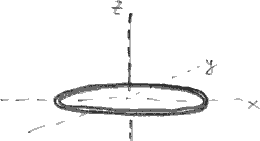
\includegraphics[width = 0.3\textwidth]{loopantenna_diagram}
  \end{center}
  \begin{enumerate}[(a)]
    \item What is the magnetic flux, $\displaystyle\Phi_{\text{mag}}(t) = \iint_{\text{disk}} \vec B \cdot d\vec a$, through the plane of the loop of the antenna?
  \interitemtext{The loop has a self-inductance $L$ and a resistance $R$.  Faraday's law for the circuit
  $$IR = -\frac{d\Phi_{\text{mag}}}{dt} - L\frac{dI}{dt}.$$
  }
    \item Assume a solution for the current of the form $I(t) = I_0\sin(\omega t - \phi)$ where $\omega$ is the angular frequency of the electromagnetic wave, $I_0$ is the amplitude of the current, and $\phi$ is a phase shift between the changing magnetic flux and the current.  Find expressions for the constants $\phi$ and $I_0$.
    \item What is the magnetic field created at the center of the loop by this current $I(t)$?
  \end{enumerate}
\section{Problem \thesection: Optional --- Magnetic monopole: experiments}
  One way to search for magnetic monopoles is by monitoring the current through a highly conductive (preferably superconducting) loop. Suppose a monopole with magnetic charge $s$ passes through a perfectly conducting circular loop with self-inductance $L$. The monopole has a constant speed $v$, perpendicular to the plane of the loop. It approaches from very far away, and then recedes to infinity. Calculate the current $I$ that flows around the loop as a result of the monopole's passage.

  \noindent (Note: experiments of this type have been running for decades, and have produced a few candidate events, but there has been no unambiguous detection.)
\section{Problem \thesection: The Director's Challenge --- Extra credit!!!}
  Formulate an interesting problem that relates a topic from 8.022 to your
  intended major or any other topic about which you are passionate.  Give references
  to help future students to understand the context.  Try to give a solution.
  Any method --- theoretical, analytical, numerical, experimental --- is acceptable.
  If you can't give a full solution, outline partial solutions. Enjoy!
\end{document}
